% Chapter 1

\chapter{Teoría de Detección de Señales} % Main chapter title

\label{Cap_SDT} % For referencing the chapter elsewhere, use \ref{Chapter1} 

%----------------------------------------------------------------------------------------

% Define some commands to keep the formatting separated from the content 
\newcommand{\keyword}[1]{\textbf{#1}}
\newcommand{\tabhead}[1]{\textbf{#1}}
\newcommand{\code}[1]{\texttt{#1}}
\newcommand{\file}[1]{\texttt{\bfseries#1}}
\newcommand{\option}[1]{\texttt{\itshape#1}}

%----------------------------------------------------------------------------------------

%Importancia del capitulo: Presentar a detalle la Teoría de Detección de Señales
En este capítulo se expone a detalle el modelo estadístico que protagoniza la presente tesis. Se trata de uno de los modelos más importantes en el desarrollo de la psicología científica y que hoy en día sigue formando parte importante del estudio de fenómenos psicológicos donde la tarea primordial de los organismos es la detección de señales específicas en su entorno para guiar su comportamiento de manera óptima.\\

%Estructura del capítulo: Exposición de supuestos, parámetros y relevancia actual.
La revisión de la Teoría de Detección de Señales comienza con una exposición de sus supuestos generales, continúa con el desarrollo de sus parámetros contemplados y su interpretación en términos de la descripción de situaciones de detección, y finalmente se ahonda en el papel que ha tenido en el desarrollo de las ciencias cognitivas y del comportamiento.\\

\section{El problema de la Detección y la Incertidumbre}

%Detectar ciertos estados en el mundo es importante para guiar nuestro comportamiento
Uno de los problemas más frecuentes a los que se enfrentan los organismos como sistemas inmersos en entornos variables y que buscan optimizar su comportamiento, es la detección de estados o eventos específicos en el mismo que le informen sobre las reglas y relaciones de contingencia vigentes.\\

%La detección es distinta de la discriminación y la categorización. Todos problemas importantes en un entorno cargado de estimulación. (El problema del embudo)
A diferencia de problemas tales como la discriminación o la categorización, situaciones donde la tarea de los organismos es evaluar la evidencia que se les presenta para asignarle una etiqueta (e.g. '¿Es A o es B?' (discriminación); 'De acuerdo a sus propeidades en tales dimensiones, se trata de un caso de...' (categorización)), cuando hablamos de un problema de detección nos referimos a situaciones que pueden plantearse en términos de preguntas 'Sí/No' (e.g. '¿La comida está buena? Sí/No', '¿Ese que viene es mi camión? Sí/No', '¿Este perro es hostil? Sí/No'), cuya respuesta permite guiar el comportamiento de los organismos en función de las consecuencias anunciadas (e.g. 'Sí, la comida está buena, me la comeré porque es seguro', 'No, ese no es mi camión, no me subiré porque acabaré en Ecatepec', 'No, no es un perro hostil, puedo acariciarlo').\\ 

%El papel del ruido
El mundo está cargado de ruido e incertidumbre. Los organismos están constantemente expuestos a distintas fuentes y tipos de estimulación en su entorno que pueden, o no, dar información relevante sobre el estado de las cosas y las reglas operantes. El primer problema que enfrentan los organismos es ordenar el caos resultante definiendo relaciones de contingencia que le permitan ajustar su comportamiento a las reglas y restricciones vigentes en su entorno. Una vez establecida la relación entre la presencia u ocurrencia de ciertos estímulos en el entorno y el acceso a ciertas consecuencias, la detección de éstos se vuelve una tarea importante para que los organismos puedan guiar su comportamiento (e.g. 'Sé que si como nueces se me cierra la garganta, ¿Hay nuez en este panqué? Si sí, no me lo como; si no, sí.').\\

%La detección de ciertos eventos no es una tarea sencilla. La información a evaluar suele ser ambigua.
Detectar 'algo' no parecería ser un problema importante si asumiéramos que dichos casos aparecen con perfecta claridad, o bien, que el organismo interesado en su detección cuenta con sensores altamente precisos que garantizan su identificación. Desafortunadamente, en el 'mundo real' las tareas de detección difícilmente se presentan así. Por lo general, la evidencia a partir de la cual juzgamos si algo está o no ocurriendo es confusa y puede llevarnos a incurrir en juicios erróneos -Falsos Positivos donde se 'detectan' casos cuando no los hay, o Falsos Negativos donde se descarta erróneamente la evidencia-. A manera de ejemplo cotidiano, imaginemos el caso de un adolescente que quiere conseguir permiso para ir de fiesta y necesita encontrar el momento ideal para pedírselo a su mamá (cuando ella esté de buen humor). Los indicadores con que cuenta el adolescente son imprecisos -los gestos, el tono de voz, las actividades que su madre realice durante el día, etc.- y errar en el diagnóstico del estado emocional de su madre y en consecuencia no obtener el permiso deseado al pedírselo en el momento inadecuado es un riesgo latente, ya sea por una mala lectura de los datos disponibles -por ejemplo, que las ansias del adolescente por salir de fiesta le hagan apresurar el momento- o bien porque los datos en sí mismos son poco claros -la mamá podría ser una persona particularmente inexpresiva o, por el contrario, terriblemente variable-.\\ 

Los organismos compensan la incertidumbre contenida en las tareas de detección con la información que poseen sobre el entorno. En términos generales, ésta puede ser de dos tipos: 1) información probabilística y 2) información sobre las consecuencias comprometidas. Sin importar a cuál de estas categorías pertenezca, los organismos construyen la 'información sobre el entorno de decisión' con base en su experiencia con el mismo y en la información que han recibido a lo largo de su vida sobre este. Por ejemplo, imaginemos el caso de un médico que trata de decidir si los resultados obtenidos en cierta prueba clínica son evidencia suficiente para diagnosticar una enfermedad 'X' a un paciente 'Y'. La evidencia con la que el médico cuenta es imprecisa: toda prueba clínica tiene un margen de error y su lectura debe complementarse con información extraída de su historia clínica por un médico especialista. El resultado de la prueba no es lo suficientemente informativo en sí mismo, el médico debe juzgar la evidencia en función de distintos factores, por ejemplo: ¿Qué tan confiable es la prueba? -¿Cuál es su tasa de aciertos y errores?-; ¿qué tan común es la enfermedad o condición cuya presencia se intenta determinar?; de acuerdo con la historia clínica del paciente, ¿qué tanto correlacionan sus características con los factores de riesgo asociados a dicha enfermedad o condición?. Es decir, el médico tiene que compensar la incertidumbre implícita en la evidencia a evaluar con toda la información probabilística de la que dispone. Y la historia no termina aquí.  Pese a que la inferencia probabilística contribuye a identificar la conclusión más probable, el médico no puede estar completamente seguro de su respuesta. Para optimizar su comportamiento y tomar la mejor decisión posible, el médico también debe tomar en consideración la información que posee sobre las consecuencias asociadas a cada escenario posible: a) Si el paciente tiene la enfermedad y el médico la detecta acertadamente, podrá tratarse a tiempo; b) Si tiene la enfermedad y el médico falla en detectarla, podría poner en riesgo su vida; c) Si no tiene la enfermedad y el médico le dice que sí, se gastarán recursos innecesarios en solucionar un problema que no existe, corriendo el riesgo de que el tratamiento le haga daño y d) Si no tiene la enfermedad y el médico decide no darle el diagnóstico, todo permanecerá igual. La tarea del médico es mucho más compleja de lo que parecía en un principio, puesto que no se limita a la lectura de una prueba clínica, sino a ponderar lo que sugieren los resultados de la misma con toda la información que posee sobre la probabilidad de las interpretaciones posibles y las consecuencias comprometidas.\\

Una vez descrito el problema de la detección, sus componentes e implicaciones para la adaptabilidad de los organismos, procederemos a desarrollar la Teoría de Detección de Señales, que permite conceptualizar este tipo de situaciones con un modelo matemático y estadístico que puede utilizarse como una herramienta -un marco conceptual- para analizar los resultados obtenidos en tareas de detección.\\

\section{Teoría de Detección de Señales}

%Origen y expansión de la Teoría de Detección de Señales en la psicología y otras áreas
La Teoría de Detección de Señales (TDS o SDT, por sus siglas en inglés) aparece por primera vez en 1954 -como tantos otros avances científicos y tecnológicos motivados por las necesidades planteadas por la Segunda Guerra Mundial- en el contexto del estudio y desarrollo de radares para detectar señales eléctricas específicas \parencite{Peterson1954}. Muy poco tiempo después, los psicólogos John A. Swets y Wilson P. Tanner contribuyeron a la expansión de la teoría a un contexto psicológico, como un modelo para estudiar la percepción de los organismos, \parencite{Tanner1954, Swets1961}. Desde entonces, la TDS constituye uno de los modelos más estudiados, desarrollados y ampliamente aplicados en Psicología, extendiéndose desde su foco inicial en el estudio de la percepción \parencite{Rosenholtz2001, Pessoa2005, Wallis2007} hacia el estudio de cualquier fenómeno o tarea donde los organismos se enfrenten al problema de emitir -y guiar su comportamiento en función a- juicios de detección ('X está'' o 'X no está'); por ejemplo, en materia de la emisión de diagnósticos clínicos \parencite{Grossberg1978, Swets2000, Boutis2010}, en el estudio de ciertas condiciones clínicas \parencite{Westermann2010, Bonnel2003, Brown1994, Naliboff1981}, en el estudio de la identificación visual de testigos \parencite{Gronlund2014, Wixted2014, Wixted2016} y un muy amplio 'etcétera' \parencite{Gordon1974, Nuechterlein1983, Harvey1992, Verghese2001}.\\ 

%La Teoría de Detección de señales como un modelo descriptivo para el problema de la detección que admite la importancia de la incertidumbre, como parte del entorno y como motor en el uso de sesgos de respuesta.
La TDS constituye un modelo estadístico que describe el problema al que se enfrentan los organismos inmersos en situaciones de detección en ambientes con incertidumbre, donde las señales -los estímulos cuya ocurrencia interesa detectar- coexisten con ruido -estímulos que no son la señal pero que pueden confundirse con esta-. Se trata de un modelo de decisión que entiende la 'detección de señales' como una tarea de elección, donde los organismos no responden simplemente con base en lo que observan, sino que eligen el juicio de elección que les permita guiar su comportamiento de la manera mas óptima posible dada la información que poseen sobre la estructura del entorno -probabilidades y consecuencias-, a la luz de la evidencia observada.\\

La generalizabilidad del modelo de la TDS al estudio de distintos fenómenos y tareas de detección se debe a lo abstracto de sus elementos: la 'señal' a detectar puede ser desde un estímulo concreto -una luz o un tono- hasta la pertenencia a una categoría -una enfermedad o amenaza- y el 'ruido' es simplemente todo elemento presente en el entorno de la tarea que no sea la señal.\\ 

\subsection{Supuestos generales del modelo}

%La TDS distingue dos grandes factores en la emisión de un juicio o respuesta: La discriminabilidad y el sesgo.
La TDS funciona como una herramienta -o marco de análisis- para traducir el desempeño observado en tareas de detección -los aciertos y errores cometidos- en inferencias sobre la precisión con que la señal se distingue del ruido (la discriminabilidad) e indicadores de la posible preferencia, o tendencia, a responder en favor o en contra de su detección (el sesgo). Esta distinción entre la Discriminabilidad de los estímulos comprometidos y el Sesgo del sistema como factores que interactúan en la emisión de juicios de detección, es una de las principales propiedades de la TDS, cuya importancia e implicaciones se discuten a continuación:\\

\begin{itemize}
  \item{El papel de la Discriminabilidad: Siempre hay incertidumbre}

%Hay variabilidad en todos los estímulos implicados en las tareas de detección (en la señal y en los estímulos no-señal)
Se habla de la detección de señales como un problema de adaptación porque se asume que la variabilidad en la presentación y percepción de los estímulos en el ambiente merma la capacidad de los organismos de emitir juicios de detección que reflejen el estado del mundo con certeza. Y dado que los estímulos-señal coexisten en el mundo con estímulos-ruido, saber qué tan saliente suele ser la presentación de una señal respecto del ruido es uno de los factores más importantes para determinar qué tan difícil es su detección para los organismos. En términos de la TDS, dicha dificultad se identifica como 'la discriminabilidad' de la tarea.\\

La discriminabilidad constituye el primer gran componente en la emisión de un juicio de detección óptimo -que refleja el verdadero estado del mundo y permite al organismo anticiparse a las consecuencias operantes-, de acuerdo con la TDS y se explica en términos de:\\ %  1) la variabilidad intrínseca en la presentación de las señales y 2) el ruido con que ésta coexiste.\\

    \begin{itemize}
      \item{1) La Variabilidad en la Señal}\\

%Existe variabilidad en la forma en que percibimos los estímulos que nos rodean. Los sistemas sensoriales y perceptuales se comportan como instrumentos de medición (error de medida)
La noción de variabilidad ha sido uno de los principales motores para el desarrollo de modelos estadísticos en Psicología. Desde que Fechner extendiera las ideas planteadas por Gauss sobre la incertidumbre contenida en toda medición -la idea de que toda medición realizada contiene el valor 'verdadero' de aquello que se quiere medir más un 'error' aleatorio que la carga de incertidumbre- al estudio de la percepción -conceptualizando nuestros sistemas sensoriales y perceptuales como 'instrumentos de medición' que perciben las cualidades 'verdaderas' de los estímulos más un 'error' en cada observación- \parencite{Fechner, Gauss}, se sentaron las bases para el desarrollo de una amplia gama de modelos matemáticos y estadísticos en Psicofísica orientados a estudiar la relación entre las cualidades físicas -"reales"- de los estímulos y la magnitud o intensidad con que se perciben psicológicamente \parencite{Link1994}.\\

%Variabilidad en la percepción de un mismo estímulo.
En el marco de la TDS, la variabilidad se considera una propiedad intrínseca de las señales a detectar bajo el supuesto de que ningún estímulo se percibe o se presenta de manera idéntica en cada exposición. Por ejemplo, imaginemos los siguientes casos: \\

\begin{itemize}

\item Una persona es expuesta a un mismo tono en 100 ocasiones distintas y después de cada una, le asigna un valor a la intensidad percibida. La intensidad percibida y reportada en cada ensayo será una mezcla entre el valor real del tono y un error aleatorio; es decir, se acercarán al valor real del estímulo pero se alejarán del mismo con cierta dispersión. A manera de ilustración, observemos la Figura~\ref{fig:Senal_percepcion}. Imaginemos que el estímulo presentado tiene un valor real de 10. En cada presentación, es muy probable que el valor percibido coincida con su valor real -la media de la distribución, $\mu$, señalada con una línea vertical roja-, pero también es posible que el valor percibido caiga por encima o por debajo de este, con cierta dispersión -las colas de la distribución-. \\

\item Supongamos que existe una escala clínica diseñada para aportar evidencia para el diagnóstico de la Depresión. Por lo general, todas las pruebas clínicas sugieren que el diagnóstico se haga con base en rangos de valores. No todas las personas con depresión van a obtener exactamente el mismo puntaje. La Figura~\ref{fig:Senal_presentacion} representa de manera gráfica esta idea: Existe una serie de posibles puntajes a obtener en la prueba de depresión (los valores en el eje de las x), y se sabe que las personas con depresión suelen obtener puntajes dentro de un rango específico con cierta probabilidad (la distribución azul), habiendo puntajes más comúnes -la media de la distribución, $\mu$, señalada en rojo- que otros.\\

\end{itemize}

\begin{figure}[th]
\centering
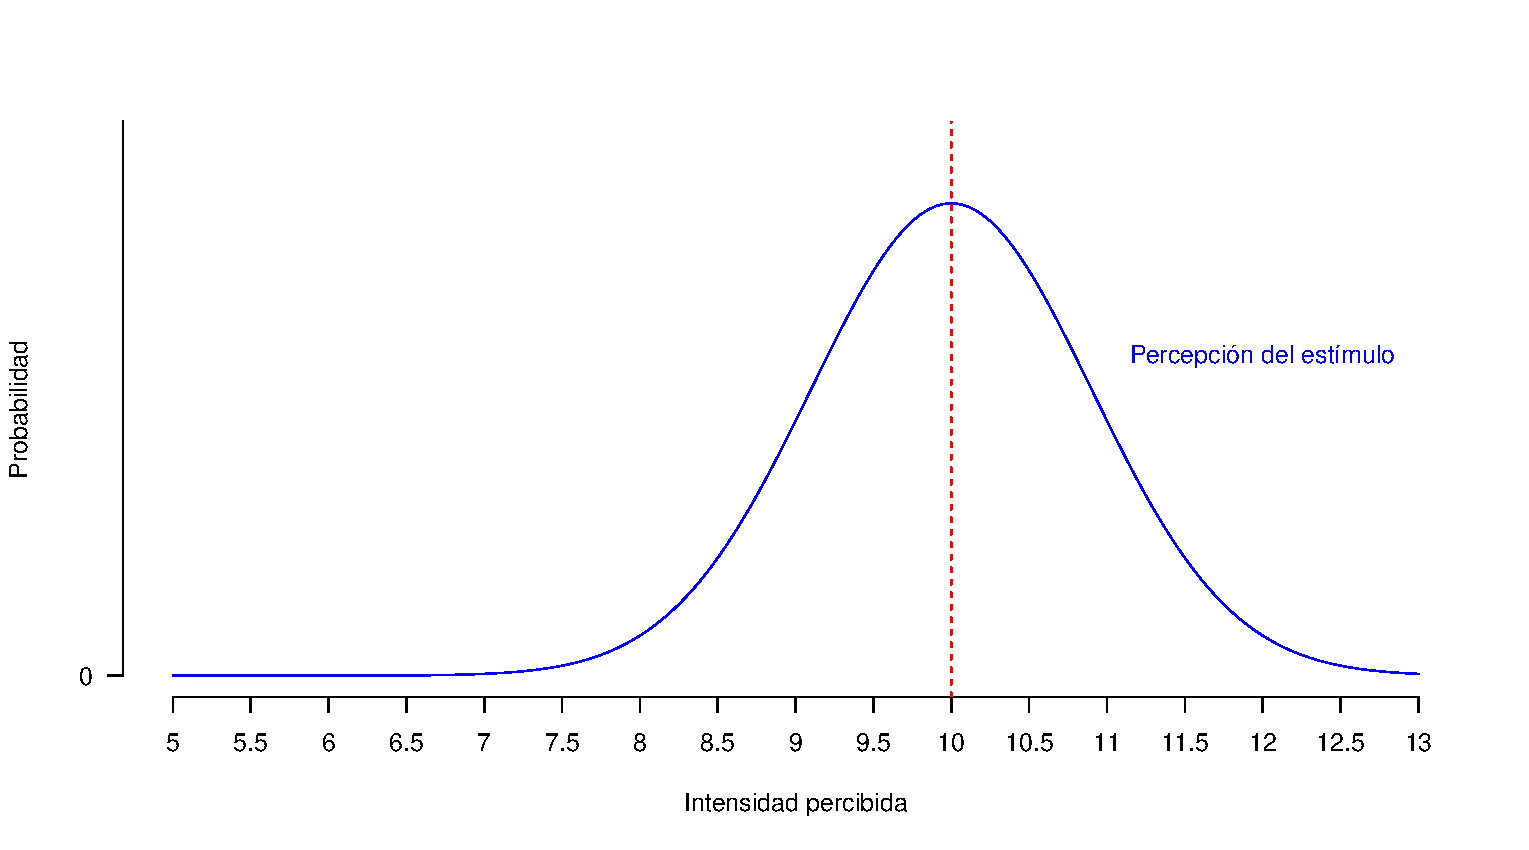
\includegraphics[width=0.80\textwidth]{Figures/Signal_Perception} 
%\decoRule
\caption[Variabilidad en la percepción de los estímulos]{Para ilustrar la idea de que las señales a detectar no son percibidas de la misma forma en cada presentación, se plantea el ejemplo de un estímulo con intensidad de 10 (la elección de valores y la omisión de unidades de medida es arbitraria). Es muy probable que el estímulo sea percibido de acuerdo a su valor real, (la media de la distribución, $\mu$) sin embargo y con menor probabilidad, también es posible que sea percibido como ligeramente más, o menos, intenso, (siendo que los valores que más se alejan del valor 'real' son menos probables que los cercanos).}
\label{fig:Senal_percepcion}
\end{figure}

\begin{figure}[th]
\centering
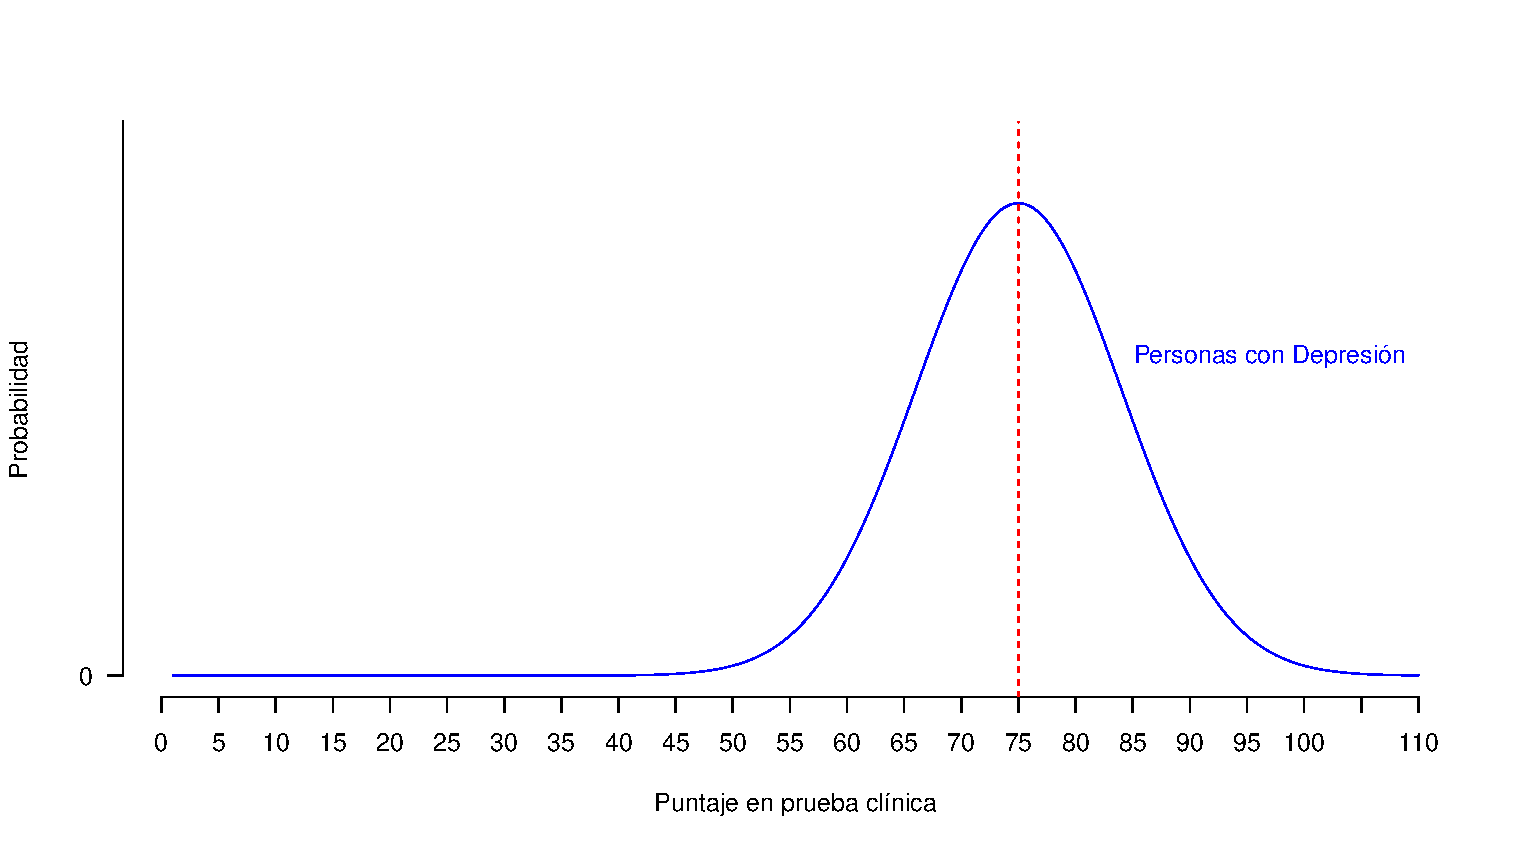
\includegraphics[width=0.80\textwidth]{Figures/Signal_Presentation} 
%\decoRule
\caption[Variabilidad en la presentación de los estímulos]{Para ilustar la idea de que las señales a detectar no se presentan de la misma forma en cada ocasión, se plantea como ejemplo la detección de una condición clínica. La figura captura la noción de que en una prueba clínica diseñada para detectar casos de Depresión, esta no se identifica a partir de un sólo puntaje sino que existe un rango de valores que se asocian a dicha condición con mayor o menor probabilidad, al rededor de un valor promedio ($\mu$, señalado en rojo). Los valores representados son arbitrarios.}
\label{fig:Senal_presentacion}
\end{figure}

En general, las Figuras~\ref{fig:Senal_percepcion} y \ref{fig:Senal_presentacion} representan el supuesto más elemental descrito en la TDS: la variabilidad es intrínseca a la presentación de los estímulos, ya sea porque nuestros sistemas sensoriales no los capturan igual en cada presentación, o porque los estímulos no se nos presentan exactamente de la misma forma en cada ocasión. En otras palabras, las señales que los organismos necesitan detectar en su entorno para guiar su comportamiento son variables, en tanto que no se presentan ni son percibidas exactamente iguales en cada ocasión.\\

      \item{2) La variabilidad en el Entorno: Ruido}\\

%La señal coexiste con el ruido y puede llegar a confundirse con el mismo.
Además de la variabilidad contenida en las señales, es necesario tomar en cuenta que estas coexisten en el mundo con otros estímulos o estados, mismos que pueden producir evidencia similar a las señales y ser por tanto, confundidos con las mismas. Por ejemplo, retomemos el caso de la prueba clínica para detectar casos de Depresión. Las pruebas clínicas psicológicas se aplican para distinguir entre las personas con cierta condición -la señal- y las que no la tienen -el ruido-. Y habíamos mencionado ya que las personas con depresión no obtienen un mismo puntaje en la prueba, sino que existe un rango de valores asociados a dicha condición con mayor o menor probabilidad. De la misma forma, al aplicar la prueba a personas que no tienen depresión tampoco se obtiene siempre el mismo puntaje, sino que el resultado obtenido suele presentarse dentro de un rango de valores distinto con su propia distribución de probabilidad. Esta extensión del ejemplo original se presenta en la Figura~\ref{fig:Noise}, donde nuevamente tenemos una distribución de probabilidad que señala los puntajes asociados con la condición a detectar (en azul) y una nueva distribución que señala los puntajes que las personas sin depresión suelen obtener al resolver la prueba con distinta probabilidad (en negro).\\

La Figura~\ref{fig:Noise} ilustra otros dos puntos claves considerados en la TDS. El primero, es que las señales no se presentan de manera aislada en el entorno, sino que suelen estar acompañadas de otros estímulos o estados del mundo -que constituyen lo que se conoce como 'ruido'-. El segundo, es que el ruido -al igual que las señales- es variable y puede llegar a presentarse o percibirse de la misma forma en que lo puede hacer la Señal. Este último punto se ilustra en la Figura con el área de las distribuciones presentadas donde estas se sobrelapan, relacionando los mismos valores con ambos estados del mundo -Depresión vs No depresión- con distinta probabilidad. Por ejemplo, parece ser que es posible observar un puntaje de 55 en una persona con o sin depresión, sin embargo, es mucho más probable observar este puntaje en ausencia de dicha condición (según la intersección entre el puntaje y cada una de las distribuciones); lo mismo ocurre con un puntaje de 65, es posible observarlo en ambos casos y sin embargo, es mucho más probable que se presente en una persona con depresión.\\

\begin{figure}[th]
\centering
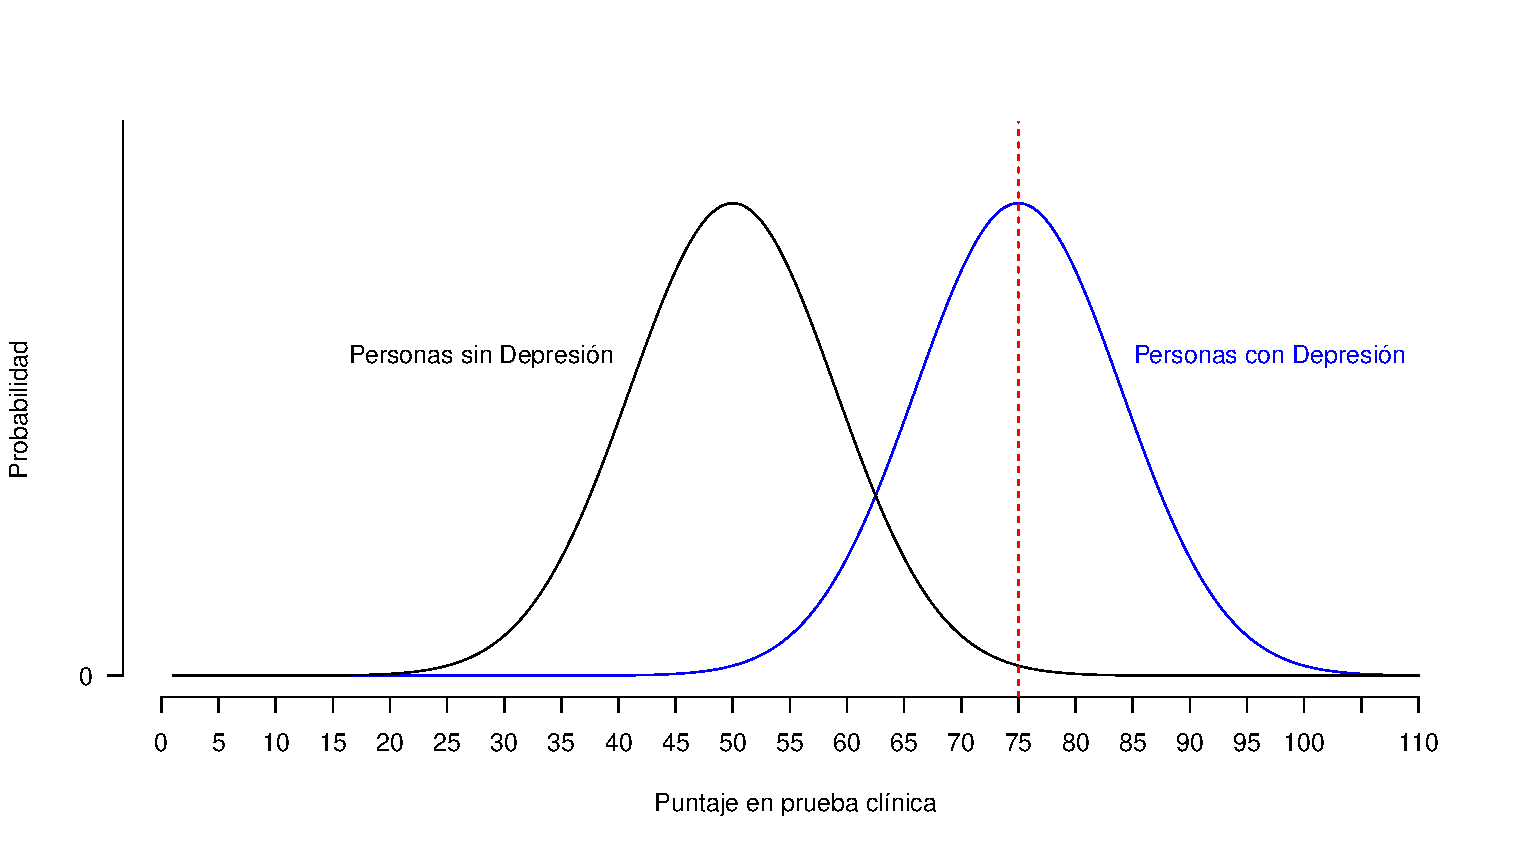
\includegraphics[width=0.80\textwidth]{Figures/Noise} 
%\decoRule
\caption[Variabilidad en la señal y en el ruido]{Para ilustar la idea de que las señales a detectar no se presentan de la misma forma en cada ocasión, se plantea como ejemplo la detección de una condición clínica. La figura captura la noción de que en una prueba clínica diseñada para detectar casos de Depresión, esta no se identifica a partir de un sólo puntaje sino que existe un rango de valores que se asocian a dicha condición con mayor o menor probabilidad, al rededor de un valor promedio ($\mu$, señalado en rojo). Los valores representados son arbitrarios.}
\label{fig:Noise}
\end{figure}

Es importante señalar que la distribución-Señal se sitúa siempre por encima de la distribución-Ruido -a su derecha-. Esto tiene sentido porque, como recordaremos las tareas de detección implican darle respuesta a una pregunta binaria 'Sí/No' respecto a la presencia o ausencia de 'algo' -la señal- en el entorno, permitiendo a los sistemas guiar su comportamiento de manera óptima. Los juicios de detección se gestan en primera instancia con base en la evidencia inmediatamente disponible. Sea cual sea la evidencia -representada de manera gráfica en el eje X sobre el cual se despliegan las distribuciones ruido y señal-, se espera que la Señal tenga 'más' de dicha evidencia que el Ruido, en tanto que este último implica la ausencia de la Señal a detectar.\\


     \end{itemize}

Tomando todo esto en consideración la discriminabilidad puede definirse en términos de las propeidades intrínsecas de los estímulos o la capacidad del sistema detector.

El soporte de las distribuciones, identificado en la Figura 1 bajo el nombre de ‘Evidencia’ rara vez se define con precisión,  teniendo una concepción más bien abstracta; La idea general es que cuando queremos detectar una señal particular, comenzamos a recolectar un tipo de evidencia específico a la tarea ante la que nos encontramos. Lo más importante, es que la señal siempre va a estar asociada en mayor medida con dicha evidencia, distribuyéndose siempre en valores situados por encima (a la derecha, en la Figura 1) del ruido.\\
 
  \item{El papel del Sesgo: La detección es decisión}\\

Una consecuencia directa de la variabilidad involucrada en el entorno de decisión, es que el desempeño de todo sistema de detección es propenso a cometer errores y emitir un juicio de presencia o ausencia de la señal, que puede no coincidir con el estado del mundo. Dependiendo la correspondencia entre el estado del mundo y el juicio emitido por el sistema de detección, la TDS maneja las clasificaciones de respuesta mostradas en la Tabla~\ref{fig:Mat_Output}; donde las celdas 2 y 3, corresponden a los errores posibles.\\

\begin{figure}[th]
\centering
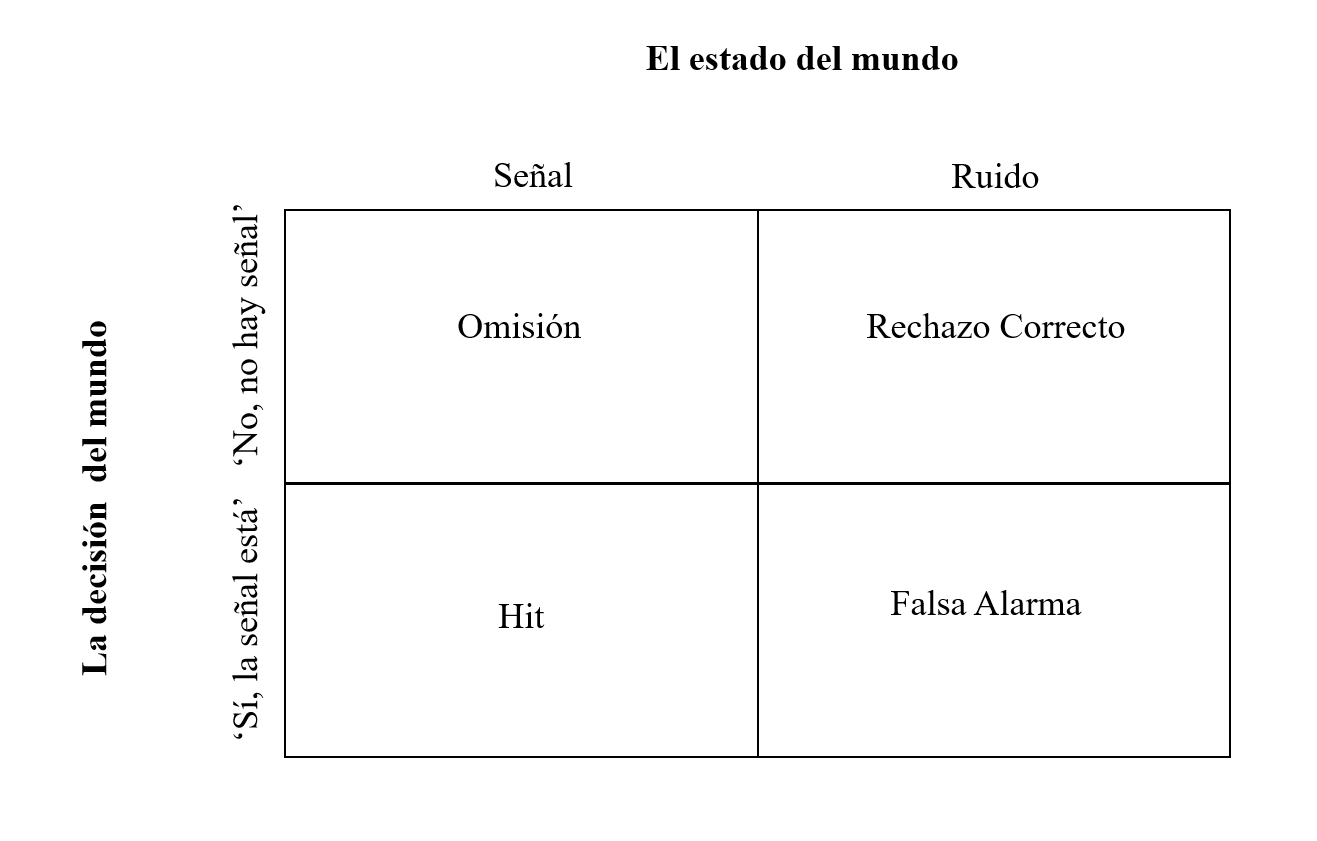
\includegraphics[width=0.60\textwidth]{Figures/Matriz_Outputs} 
%\decoRule
\caption[Posibles Resultados a obtener en una Tarea de Detección]{}
\label{fig:Mat_Output}
\end{figure}

La TDS asume que el organismo fija un criterio de elección a lo largo del eje de la Evidencia, que va a determinar a partir de cuánta evidencia va a juzgar la señal como presente. Dicho criterio se va a representar como una línea transversal que atraviesa ambas distribuciones en una determinada altura, y se le va a identificar con el parámetro k. La TDS asume que los organismos van a fijar esta regla de elección, ponderando la información a la que tienen acceso con la información que poseen sobre la estructura de la tarea (i.e. cómo suele presentarse la señal, qué tan probable es que se presente, etc.)\\

    \begin{itemize}
      \item{Los errores cuestan y los aciertos pagan: Matrices de pago}\\

      \item{Estimados de Probabilidad}

      \item{Sesgo o Preferencial}\\

  El sesgo se define como la preferencia del sistema a emitir respuestas de un tipo particular (i.e. 'Sí, detecto la señal' o 'No, no está'). La TDS cuenta con dos parámetros dedicados a la medición y evaluación del sesgo de los sistemas sometidos a tareas de detección.

 Sin embargo, no todos los errores tienen el mismo costo. Imaginemos el caso de una presa en potencia que busca determinar si el sonido que acaba de escuchar en la maleza corresponde o no con el de un depredador; no hay tiempo que perder, y el costo que dicho organismo tendría que pagar por cometer una falsa alarma (gasto innecesario de energía) o una omisión (morir devorado) es sustancialmente diferente. En este escenario particular, es muy probable que la presa sea mucho más propensa a correr por su vida, juzgando la presencia del depredador a partir de valores menores de evidencia.\\

Esta discrepancia en el peso que se le da a las consecuencias posibles de emitir una u otra respuesta y obtener uno de los cuatro posibles resultados, suele representarse en términos de una matriz de pagos, que nos ayude a definir cuáles son las consecuencias que el organismo buscará evitar o promover, según sea el caso, en mayor medida.\\

Ya sea por los distintos pesos que tengan las posibles consecuencias para el organismo, o porque se tiene una preferencia o predisposición inherente a decretar la presencia o ausencia de la señal, la TDS asume que el desempeño de los organismos que se enfrentan a tareas de detección de señales va a depender tanto de la calidad de la información a la que se tiene acceso (dentro de lo que se incluye la importancia de la variabilidad, que determina tanto la discriminabilidad de la señal como la sensibilidad del sistema ante la misma), como de un sesgo de elección.\\

La localización del criterio en nuestro eje de evidencia recolectada va a estar altamente influida por el sesgo que tenga nuestro sistema. Podemos hablar entonces de dos tipos distintos de sesgo: conservador y liberal. El primero, favorece la emisión de respuestas negativas al desplazar el criterio a la derecha y requerir al sistema la recolección de mayores niveles de evidencia antes de dar por detectada la señal. El segundo, promueve la detección de la señal, situando el criterio de elección hacia la izquierda, emitiendo un juicio de detección con valores menores de evidencia. Nótese que un sistema carente de sesgo, sería aquel que situara su criterio de elección justo en el punto en que las dos distribuciones se juntan, donde la probabilidad de cometer cualquiera de los tipos de acierto y errores, son iguales entre sí.\\

     \end{itemize}
\end{itemize}

\subsection{Parámetros del modelo}

Como se mencionó previamente, al realizar una tarea de detección existen dos posibles tipos de aciertos: al detectar la señal (Hits) y al rechazar el ruido (Rechazos), y dos posibles tipos de errores: los falsos positivos (Falsas alarmas) y los falsos negativos (Omisiones). La materia prima con base en la cual funciona el modelo propuesto por la TDS, son las tasas de aciertos y errores cometidos durante la tarea, de manera que por cada participante que pasa por una tarea de detección, tenemos cuatro tasas que describen su ejecución:

La Tabla 2 ilustra el cómputo de las cuatro tasas de ejecución, como una relación entre el resultado obtenido y el tipo de ensayo con base en el que se le definió como tal. Es decir, tenemos dos tasas definidas en relación al número total de ensayos con la señal (la tasa de hits y la tasa de omisiones) que nos dicen qué proporción de los ensayos con señal fueron detectados correctamente y cuáles se dejaron pasar; y tenemos dos tasas definidas en relación al total de ensayos con ruido (la tasa de falsas alarmas y la tasa de rechazos correctos) que nos describen la relación de los ensayos con ruido que fueron discriminados correctamente y aquellos que se confundieron con la señal.

Para realizar el análisis de datos, bajo el marco de la TDS, sólo necesitaremos un par de estas tasas: la tasa de hits y la tasa de falsas alarmas. Esto bajo el entendido de que las tasas de omisión y rechazos correctos no son más que su complemento, respectivamente, y que estas dos tasas contienen toda la información que necesitamos sobre el desempeño de los participantes.

La idea general de la importancia de estas tasas de ejecución, es que cada una representa el área de las distribuciones de ruido y señal que cae a la izquierda o derecha del criterio de decisión.

Para la estimación paramétrica se utiliza la misma lógica, pero se sigue el procedimiento inverso. Dado que no podemos observar ni cuantificar de manera directa el criterio usado por los participantes para responder a la tarea, qué tan juntas o separadas se encuentran las distribuciones de ruido y señal para cada participante o qué tipo de sesgo pudieran estar siguiendo, utilizamos las tasas de ejecución para hacer inferencias sobre la localización del criterio, la diferencia entre las medias de ambas distribuciones y el grado en que una respuesta se favorece sobre otra. 

A partir de ahora comenzaremos a hablar sobre cómo se calculan cada uno de los parámetros del modelo, de acuerdo a la teoría clásica que sigue los supuestos estadísticos previamente descritos.  Es importante aclarar que el Graficador de Tasas previamente expuesto no representa la teoría con entera precisión; el propósito de ese primer Graficador es simplemente ilustrar cómo describe la TDS el comportamiento de un sistema que se enfrenta ante una tarea de detección, donde existen dos distribuciones que se sobreponen. El Graficador permite manipular directamente la localización del criterio, con la simpleza que implicaría desplazar una línea vertical sobre el eje de decisión y ver qué consecuencias tiene sobre la probabilidad de obtener un tipo particular de acierto o error.


Antes de ahondar a detalle en los parámetros, hay que declarar un par de supuestos formales que hace la Teoría para facilitar la representación gráfica del modelo y la estimación paramétrica:

\begin{enumerate}
\item En su forma clásica, la TDS asume que las distribuciones de ruido y señal son distribuciones normales.
  \begin{itemize}
  \item 
  \end{itemize}
\item En su forma estándar, se asume que las distribuciones de ruido y señal son equivariantes, (compartiendo una desviación estándar de 1).
  \begin{itemize}
  \item 
  \end{itemize}
\item La distribución de ruido tiene su media en 0. 
  \begin{itemize}
  \item La estimación de todos los parámetros del modelo de detección de señales se hace tomando como referencia la distribución del ruido (con  media 0 y desviación estándar de 1)
  \end{itemize}
\end{enumerate}



\begin{itemize}
\item Discriminabilidad $(d')$

La disc

La discriminabilidad se representa en los modelos de detección de señales con un parámetro $d'$, que representa la distancia entre las medias de las distribuciones de ruido y señal. 

Para encontrar la distancia entre las medias de la distribución de ruido y señal, necesitamos saber el punto en que el criterio toca cada distribución. Para ello, calculamos las probabilidades complementarias a las tasas de hits y falsas alarmas y las traducimos a puntajes Z (Ver Fig. 3). Dado que el puntaje Z funciona como una medida de dispersión de la media, basta con restar el puntaje Z de la intersección del criterio con la distribución de señal a el puntaje Z de intersección con la distribución de ruido para conocer la localización de la media de la señal. Por definición, d’ sólo puede tener valores positivos ya que la teoría asume que la distribución de señal siempre está a la derecha de la distribución de ruido porque contiene una mayor cantidad de la evidencia con base en la cual se hace el juicio de detección de la señal.



\item Criterio  $k$

Una vez que hemos resumido el desempeño de nuestro participante en la tarea de detección, el parámetro cuya estimación resulta más sencilla y directa es el Criterio (k). Entender cómo se computa el parámetro nos requiere únicamente de mantener presente el supuesto de que el Ruido se distribuye normalmente y se va a localizar siempre a la izquierda de la señal, por lo que le asignamos una media de cero para tener un punto de referencia para estimar el espacio en que se desarrollan el resto de los parámetros. \\

Para calcular el criterio lo único que necesitamos es conocer la tasa de Falsas Alarmas, que tal y como mencionábamos en el segmento anterior, nos indica qué proporción de la distribución de ruido cae a la derecha del criterio. Dado que a la distribución de ruido, le fue asignada arbitrariamente una media de cero, podemos asignar un valor al punto en que el criterio corta la distribución de ruido y define las tasas de Rechazos y Falsas Alarmas obtenidas por el participante. Conociendo el área de la distribución de Ruido que cae bajo el criterio, (el complemento de la tasa de Falsas Alarmas, o bien, la Tasa de Rechazos correctos), y sabiendo que la distribución tiene una desviación estándar de 1, podemos convertir el valor de la tasa (que corresponde a la probabilidad de cometer un rechazo correcto, de acuerdo al área bajo la curva) en Puntajes Z y conocer la localización del criterio.\\

 El parámetro k, por lo general, va estar representado por un número natural (un número positivo), que indica en términos de Puntajes Z  la posición del criterio sobre el eje de decisión, relativo a la distribución de ruido con media cero. El criterio sólo tiene valores positivos, porque normalmente se espera que la tasa de falsas alarmas nunca tenga un valor mayor a 0.5 (las consecuencias de una tasa de Falsas Alarmas tan alta, se expondrán con más claridad en el apartado correspondiente a la d’. \\


\item Sesgo - $\beta$

El parámetro más comúnmente utilizado en la literatura para evaluar el sesgo de los participantes en estudios donde se aplica el modelo de detección de señales al análisis de tareas experimentales, es Beta ($\beta$). Se define como una razón entre la probabilidad con que la evidencia  \\

$\beta = \frac{p(Signal)}{p(Noise)}$

si $\beta<1$ o C<0, sabemos se trata de un sesgo liberal y si $\beta>1$, C>0, hablamos de un sesgo conservador.\\

\item Sesgo - $C$


\end{itemize}   %Terminan los parametros



%----------------------------------------------------------------

\subsection{Tareas de detección}

\begin{itemize}
\item Tareas de detección binaria 

En el laboratorio, la  TDS se estudia a partir  de tareas de detección donde se expone a un  sujeto  a  N  número  de  ensayos,  (comprendidos  por  n  ensayos con  sólo  ruido  y  n  ensayos donde  el  ruido  viene  acompañado  de  la  señal)  ante  los  que  se  le  pide  al  participante  que responda eligiendo una de dos opciones: Sí está la señal o No está la señal. En estos escenarios controlados,  el  experimentador  decide  la  proporción  de  ensayos  con  y  sin  señal  que  se presentarán, así como la matriz de pagos que definirán la utilidad de sus aciertos y errores. \\


\item Tareas con escala de confianza

Un segundo procedimiento comúnmente utilizado en tareas de detección implica añadir un paso adicional a la tarea de los participantes. 

\parencite{McNicol}

\item Tarea con elección forzada entre dos alternativas.



\end{itemize}

